\documentclass[a4paper, 12pt]{article}

\usepackage[english, russian]{babel}
\usepackage[T2A]{fontenc}
\usepackage[utf8]{inputenc}
\usepackage{mathtext}
\usepackage{amsfonts}
\usepackage{ amssymb }
\usepackage{amsmath}
\usepackage{graphics}
\usepackage{graphicx}
\usepackage{wrapfig}
\usepackage{geometry}
\usepackage{float}
\geometry{
	a4paper,
	total={170mm, 257mm},
	left=20mm,
	top=10mm}

\title{Лабораторная работа 3.2.4 и 3.2.5. \\ Свободные и вынужденные колебания в электрическом контуре}
\author{Абакшин Василий, Б05-207}
\date{3 сентября 2023 г.}
\begin{document}
	\maketitle
	\textbf{Цель работы}: исследование свободных и вынужденных колебаний в колебательном контуре.
	
	\textbf{Оборудование}: осциллограф, генератор сигналов, магазин сопротивлений, магазин емкостей, магазин индуктивности, соединительная коробка с шунтирующей емкостью, соединительные провода.
	\subsection*{Установка}
	\begin{figure}[h]
		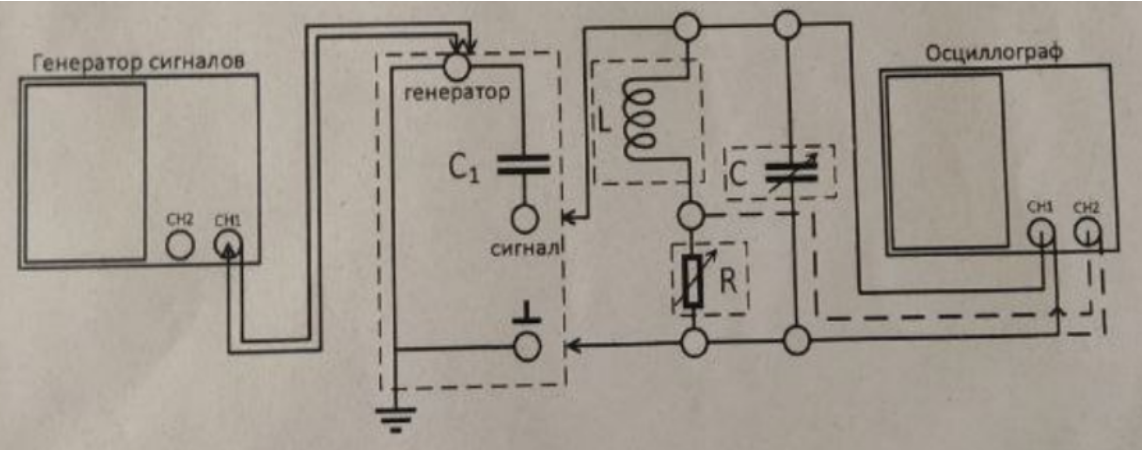
\includegraphics[width = \textwidth]{Scheme.png}
		\caption{Схема электрической цепи}	
	\end{figure}
	
	В цепи используется катушка постоянной индуктивности $L = 100 \ \text{мГн}$, переменной емкости $C$ и сопротивления $R$. Колебания напряжения наблюдаются на осциллографе, подключенном параллельно конденсатору. Также используется дополнительная емкость $C_1$, на которую изначально поступает сигнал генератора. Она нужна для снижения выходного импеданса генератора, чтобы он не сильно влиял на общий импеданс контура. 
	
	При исследовании свободных колебаний будем подавать на контур периодические импульсы, а в случае вынужденных колебаний --- синусоидальный сигнал.
	\newpage
	
	\subsection*{Ход работы и измерения}
	
	\textbf{1.} Период колебаний при установленной 0 емкости на магазине емкостей $T_0 = 64,4 \text{мкс}$. 
	
	$T_0 = 2\pi \sqrt{LC_0} \longrightarrow C_0 = \frac{T^2}{4\pi^2L} = 105,05 \cdot 10^{-11} \approx 1 \ \text{нФ} $
	
	Будем увеличивать емкость контура и сравнивать экспериментальную величину периода с вычисленной теоретически: 
	
	\begin{table}[h]
		\centering
		\begin{tabular}{|c|c|c|}
		\hline
		$C + C_0$, нФ & $T_{exp}$, мкс & $T_{th}$, мкс \\ \hline
		2 & 90,4 & 88,9 \\
		3 & 109 & 108,8 \\
		4 & 127 & 125,7 \\
		5 & 142 & 140,5 \\
		6 & 154 & 153,9 \\
		\hline
		\end{tabular}
		\caption{Экспериментальные и теоретические значения периодов колебаний}
	\end{table}
	
	\begin{center}
		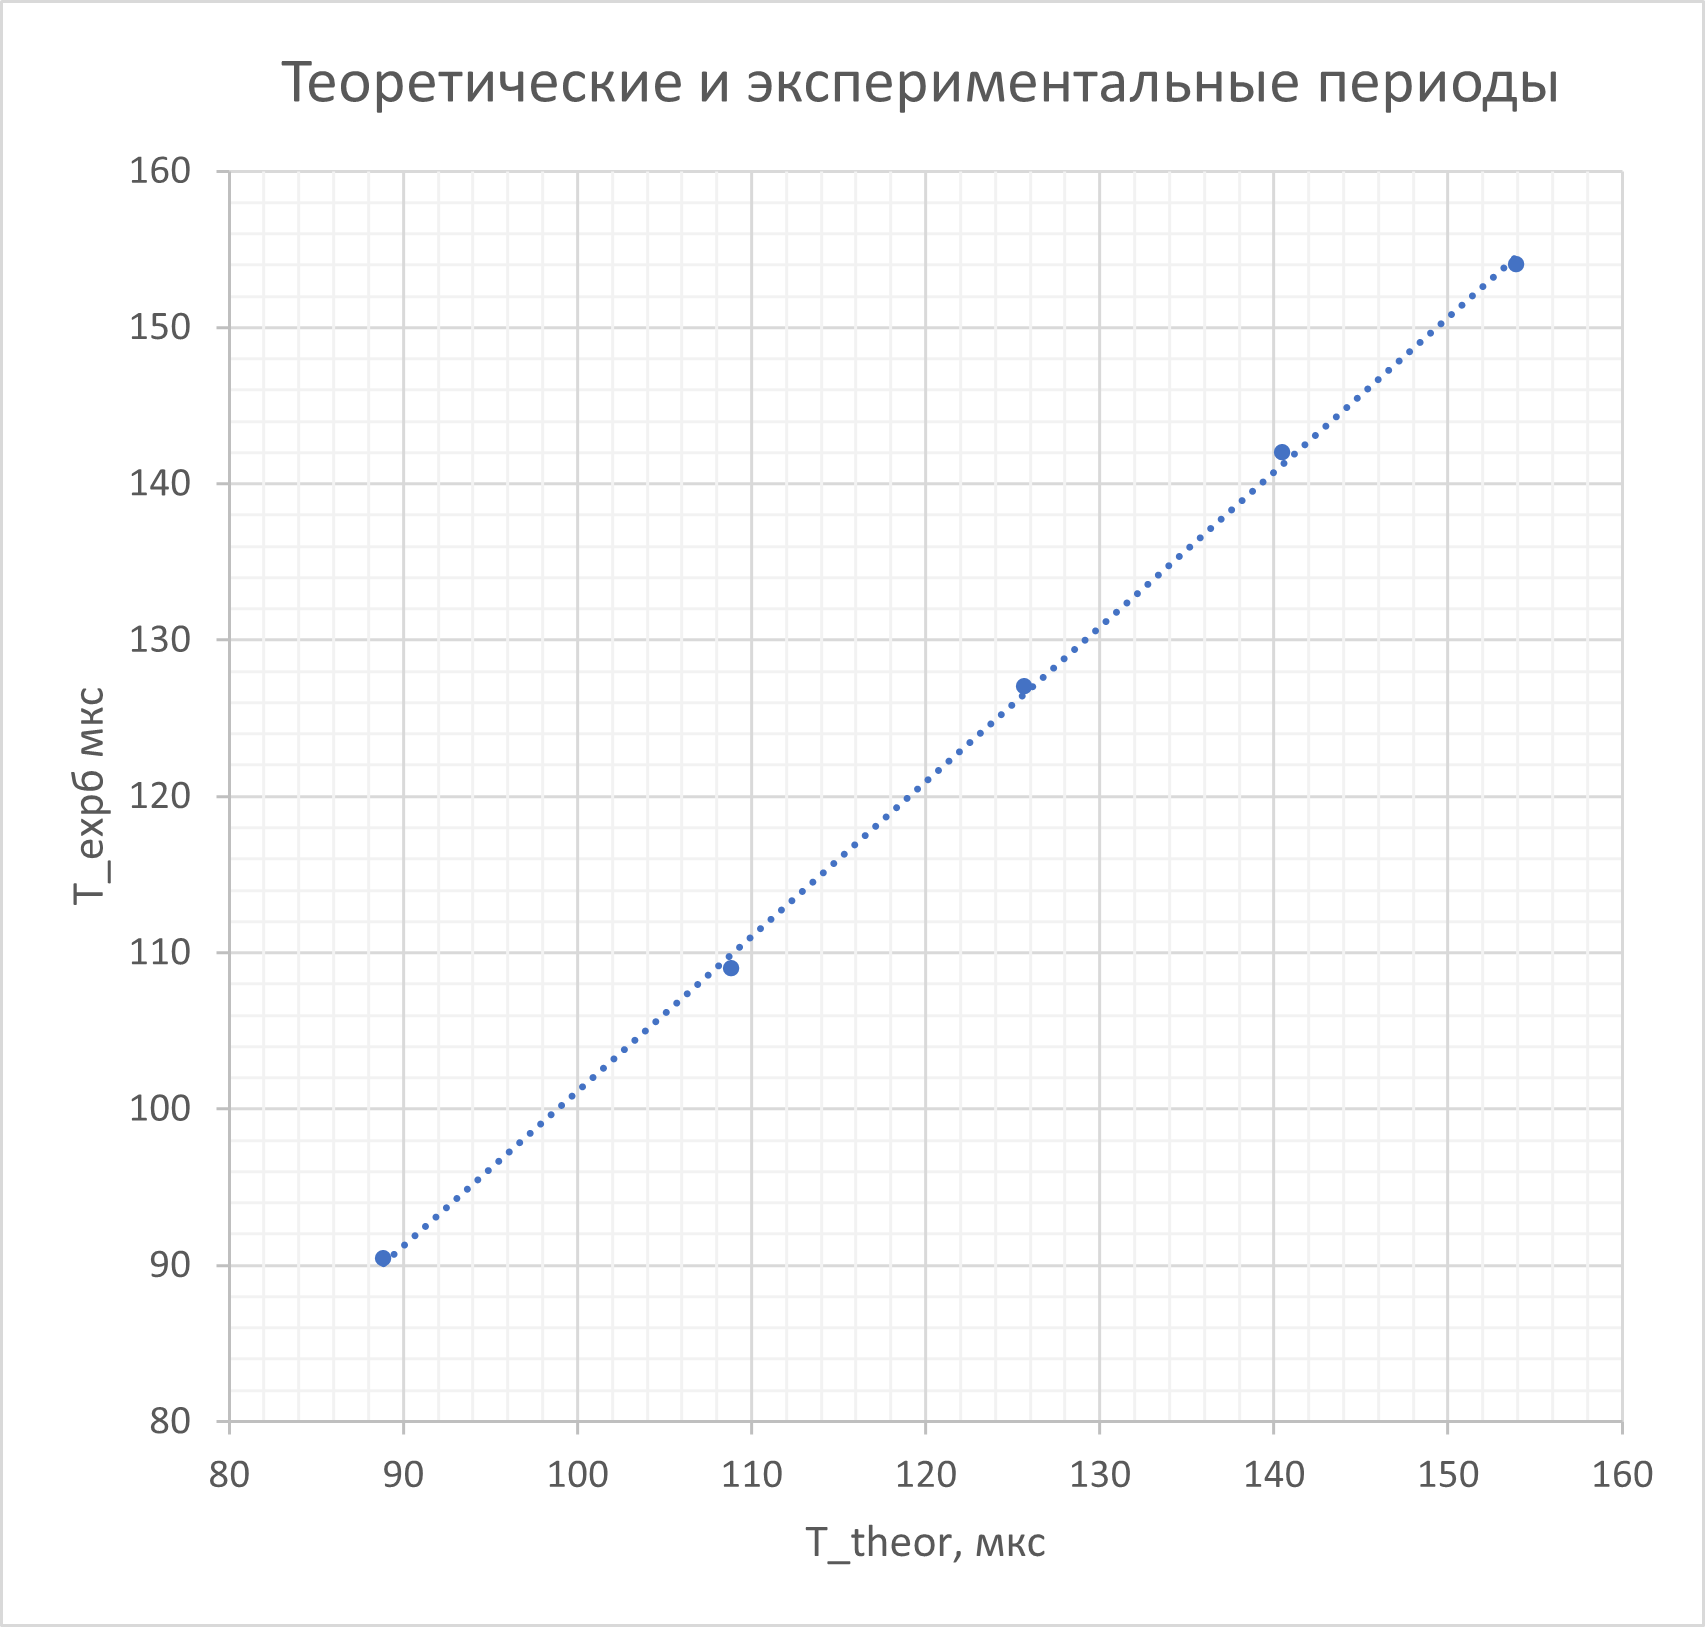
\includegraphics{Gr1}
	\end{center}
	
	Экспериментальные результаты отличаются от теоретических не более, чем на 1,7\%. Наибольший вклад в погрешность вносит точность наших измерений. Что касается графика, угол наклона $\alpha = 0,991 \pm 0,014$. То есть случайная погрешность составила $\varepsilon_{\alpha} \approx 1,5 \%$
	
	\textbf{2.} Подберем и установим значение $C^*$ так, чтобы частота собственных колебаний была $\nu_0 = 6.5$ кГц. $C^* = \frac{1}{4\pi^2\nu_0^2L} \approx 6$ нФ. Рассчитаем теоретически критическое сопротивление контура $R_{cr} = 2\sqrt{\frac{L}{C}} = 8165$ Ом. Измеряем логарифмических декремент затухания по соседним максимумам при различных внешних сопротивлениях ($0,05 R_{cr} - 0,2R_{cr}$):
	\newpage
	\begin{table}[h]
		\centering
		\begin{tabular}{|c|c|c|c|c|}
			\hline
			$R_{\text{вн}}$, Ом & $R = R_{\text{вн}} + R_L$, Ом& $\theta = \ln \frac{U_k}{U_{k+1}}$ & $Q = \frac{\pi}{\theta}$ & $\sigma_{Q}$ \\ \hline
			 408 ($0,05R_{cr}$) & 443 & 0,38 & 8,25 & 0,65 \\ \hline
			653,2 ($0,08R_{cr}$) & 688,2 & 0,54 & 5,81 & 0,32  \\ \hline
			898,2 ($0,11R_{cr}$) & 933,2 & 0,73 & 4,3 & 0,18 \\ \hline
			1143,1 ($0,14R_{cr}$) & 1178,1 & 0,92 & 3,42 & 0,11 \\ \hline
			1633 ($0,2R_{cr}$) & 1668 & 1,27 & 2,46 & 0,06 \\ \hline
		\end{tabular}
		\caption{Декремент затухания свободных колебаний}
	\end{table}
	
	Основная часть ошибки при расчете добротности данным способом --- случайная ошибка в измерении напряжения. Примем её за $2\%$. В таком случае $\sigma_{\theta} \approx 0,03$.
	
	Здесь мы приняли $R_L = 35$ Ом приблизительно.
	Построим график зависимости $\frac{1}{\theta^2} = f(\frac{1}{R^2})$. Так как
	\[\theta = \ln\left(\frac{U_k}{U_{k + 1}}\right) = \gamma T = \gamma \frac{2\pi}{\omega_1}\]
	\[\theta^2 = \gamma^2\frac{4\pi^2}{\omega_1^2} = \gamma^2 \frac{4\pi^2}{\omega_0^2 - \gamma^2}\]
	\[\frac{1}{\theta^2} = \frac{1}{4\pi^2}\left(\frac{\omega_0^2}{\gamma^2} - 1\right) = \frac{1}{4\pi^2}\left(\frac{4L}{CR^2} - 1\right)\]
	
	то зависимость должна получиться линейной:
	
	\[\frac{1}{\theta^2} = \frac{1}{R^2}\frac{L}{C\pi^2} - \frac{1}{4\pi^2}\]
	\begin{figure}[h]
		\centering
		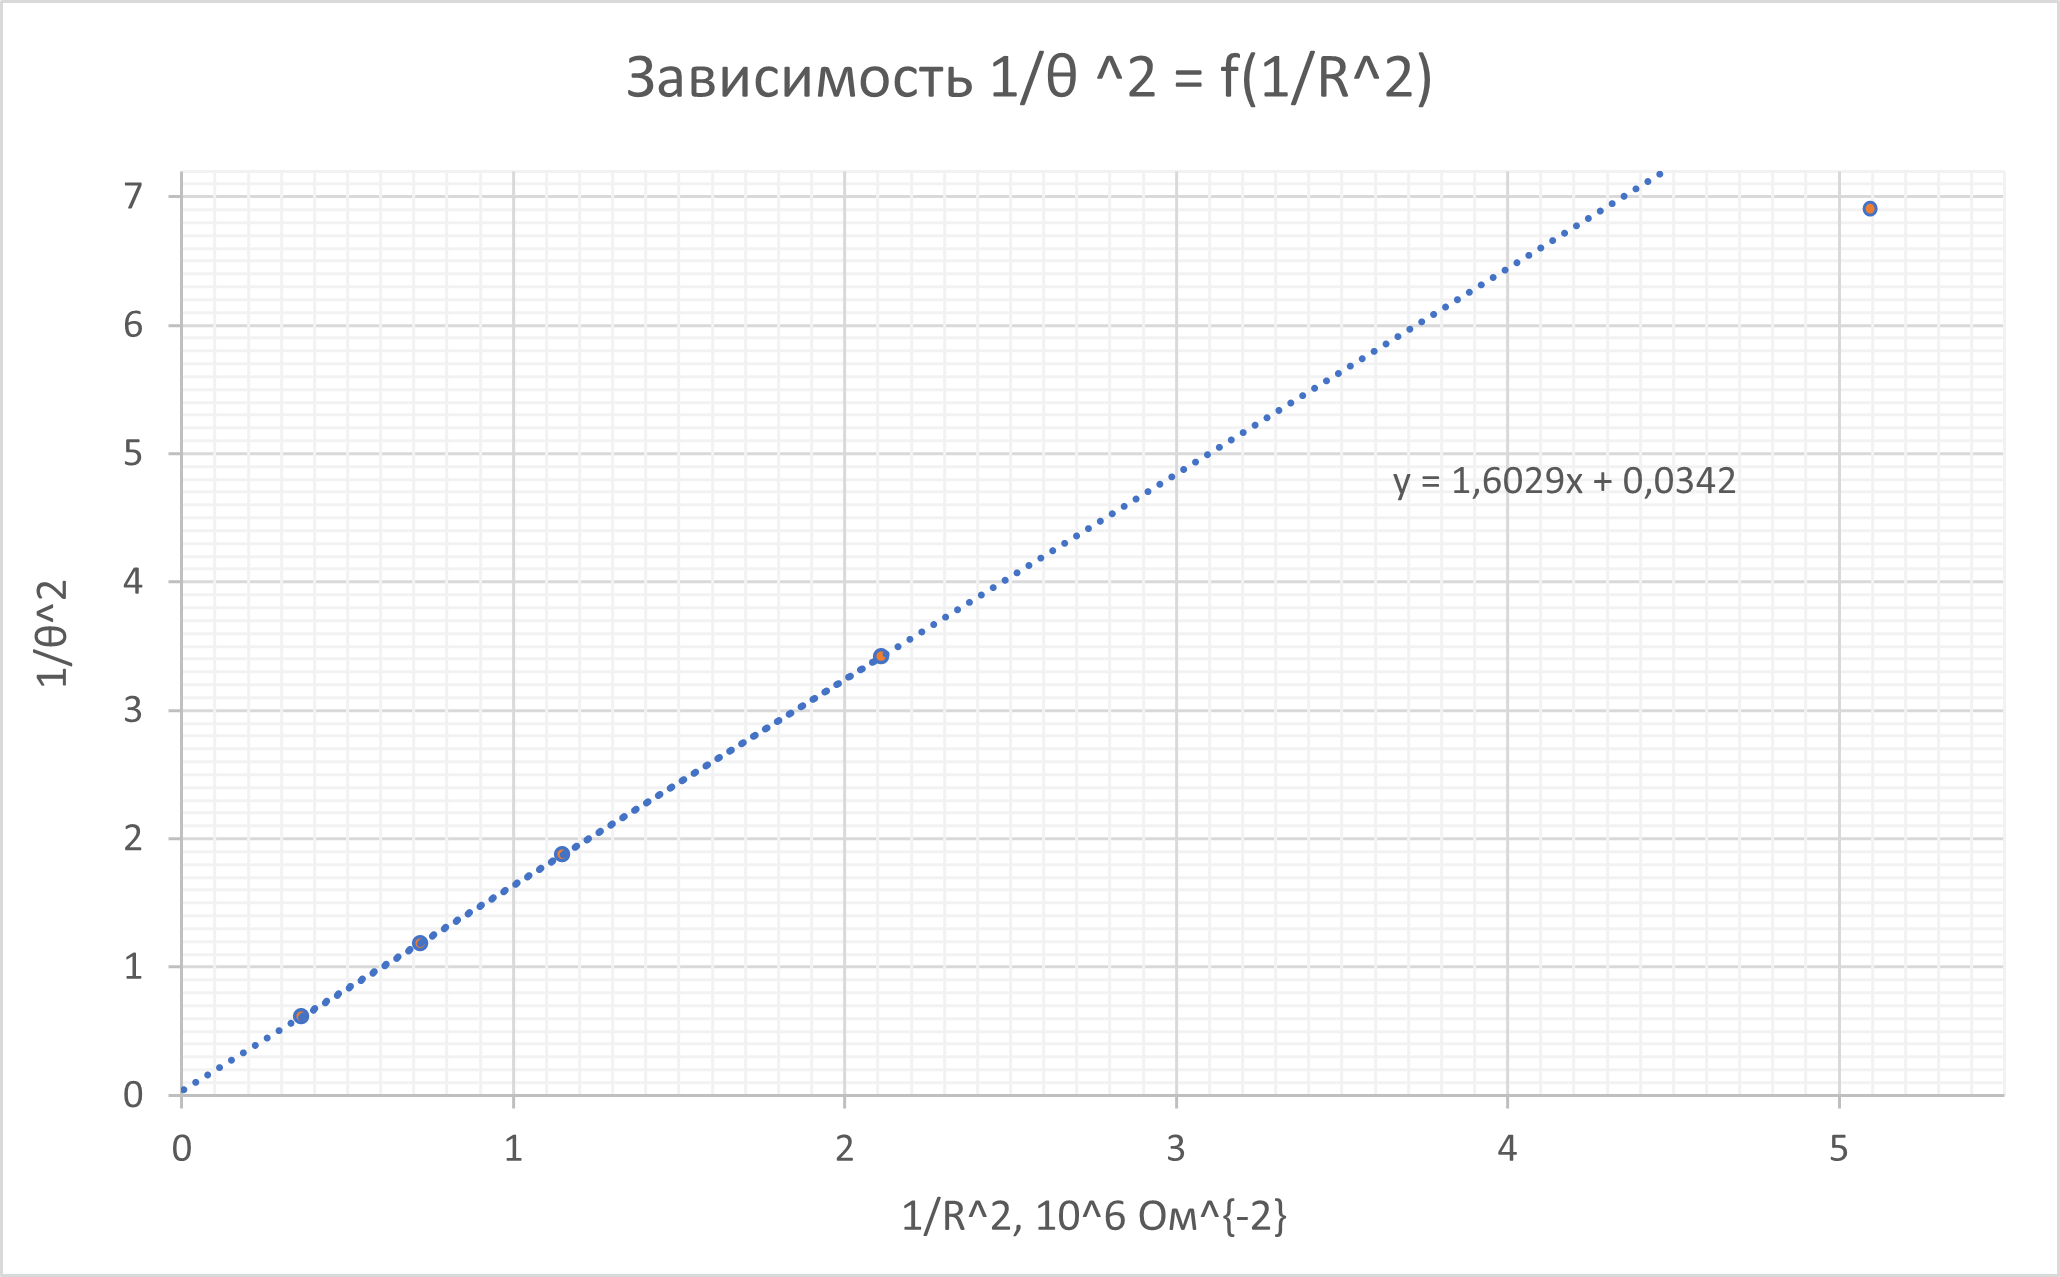
\includegraphics[width = \textwidth]{Gr2}
	\end{figure}
	
	
	Прямая построена по 4-м точкам: всем, кроме последней, её убрали из рассмотрения, так как она плохо ложиться на прямую. Коэффициент $k = (1,603 \pm 0,008)\cdot 10^6 \quad \varepsilon_k = 0,5 \%$. Найдем $R_{cr} = 2\pi \sqrt{k} = (7955 \pm 20)$ Ом. В пределах случайной погрешности не попадает в теоретически расчитанное значение, вероятно потому, что мы не очень хорошо знаем $R_L$.\\
	
	\textbf{3.} Рассчет добротности по спирали на фазовой плоскости. В помощью осциллографа получаем портрет колебаний на фазовой плоскости (в режиме XY), определяем декремент затухания по соседним пересечениям оси X. Так как измерения проводились на глаз, то оценим погрешность $\sigma_U = 0,1$ дел.
	
	\begin{table}[h]
		\centering
		\begin{tabular}{|c|c|c|c|c|c|}
			\hline
			R, Ом & $U_k$, дел & $U_{k + 1}$, дел & $\theta$ & $Q$ & $\sigma_{Q}$  \\ \hline
			443 & 4,4 & 3 & 0,38 & 8,20 & 0,86 \\ \hline
			1668 & 3,8 & 1 & 1,34 & 2,35 & 0,18 \\ \hline 
		\end{tabular}
		\caption{Определение добротности по фазовой плоскости}
	\end{table}
	
	\textbf{4.} Рассчитаем теоретическое значение добротности через параметры контура
	\[Q = \frac{\pi}{\theta} = \frac{\pi}{\gamma T} = \frac{\pi}{\frac{R}{2L}\frac{2\pi}{\omega_1}} = \frac{L}{R}\omega_1 = \frac{L}{R}\sqrt{\omega_0^2 - \gamma^2} = \frac{L}{R}\sqrt{\frac{1}{LC} - \frac{R^2}{4L^2}} = \frac{1}{2}\sqrt{\frac{4L}{CR^2} - 1}\]
	
	При параметрах $L = 100$ мГн, $C = 6$ нФ имеем (примем погрешность $\sigma_{R_L} = 5$ Ом):
	
	1. $R_1 = 443$ Ом $Q_1 = 9,20$, $\sigma_{Q_1} = 0,10$
	
	2. $R_2 = 1668$ Ом $Q_2 = 2,40$, $\sigma_{Q_2} = 0,01$\\
	
	\textbf{5.} Измерение АЧХ и ФЧХ вынужденных колебаний.
	
	Установим на генераторе синусоидальный сигнал и будем наблюдать картину вынужденных колебаний. Занесем в таблицу полученные данные и построим графики в координатах $\frac{U}{U_{0}} = \frac{\nu}{\nu_0}$
	\begin{table}[h]
		\centering
		\begin{tabular}{|c|c|c|c|}
			\hline
			$\nu$, Гц & $U$, В & $\Delta t$, мкс & $\Delta \phi$, $\cdot \pi$ \\ \hline
			5700 & 37 & 72,4 & 0,83 \\ \hline
			5800 & 42,5 & 69,2 & 0,80 \\ \hline
			5900 & 49 & 67,2 & 0,79 \\ \hline
			6000 & 57 & 62,8 & 0,75 \\ \hline
			6100 & 68 & 58,8 & 0,72 \\ \hline
			6200 & 79 & 53,2 & 0,66 \\ \hline
			6300 & 90 & 47,6 & 0,60 \\ \hline
			6400 & 99 & 40,8 & 0,52 \\ \hline
			6500 & 102 & 34,4 & 0,45 \\ \hline
			6600 & 98 & 27,2 & 0,36 \\ \hline
			6700 & 90,5 & 22 & 0,29 \\ \hline
			6800 & 82,5 & 17,2 & 0,24 \\ \hline
			6900 & 74 & 14,8 & 0,20 \\ \hline
			7000 & 66,5 & 12 & 0,17 \\ \hline
			7100 & 59,5 & 10,4& 0,15 \\ \hline
			7200 & 54 & 8,8 & 0,13 \\ \hline
			7300 & 49,5 & 8 & 0,12 \\ \hline
			7400 & 46,5 & 6,4 & 0,095 \\ \hline
			7500 & 43 & 6 & 0,09 \\ \hline
			7600 & 40 & 4,4 & 0,07 \\ \hline
		\end{tabular}
		\hspace{.06\textwidth}
		\begin{tabular}{|c|c|c|c|}
			\hline
			$\nu$, Гц & $U_{max}$, В & $\Delta t$, мкс & $\Delta \phi$, $\cdot \pi$ \\ \hline
			5600 & 22,0 & 50 & 0,56 \\ \hline
			6000 & 27,6 & 40 & 0,48 \\ \hline
			6200 & 29,6 & 35,6 & 0,44 \\ \hline
			6400 & 30,8 & 31,2 & 0,40 \\ \hline
			6600 & 31,6 & 26,8 & 0,35 \\ \hline
			6800 & 31,6 & 22,8 & 0,31 \\ \hline
			7000 & 31,2 & 19,6 & 0,27 \\ \hline
			7200 & 30,4 & 16,8 & 0,24 \\ \hline
			7400 & 29,6 & 14 & 0,21 \\ \hline
			7600 & 29,5 & 12 & 0,18 \\ \hline
			8000 & 26,4 & 8,4 & 0,13 \\ \hline
		\end{tabular}
		\caption{АЧХ и ФЧХ для $R_1 = 443$ Ом и $R_2 = 1668$ Ом}
		
	\end{table}
	
	\begin{center}
		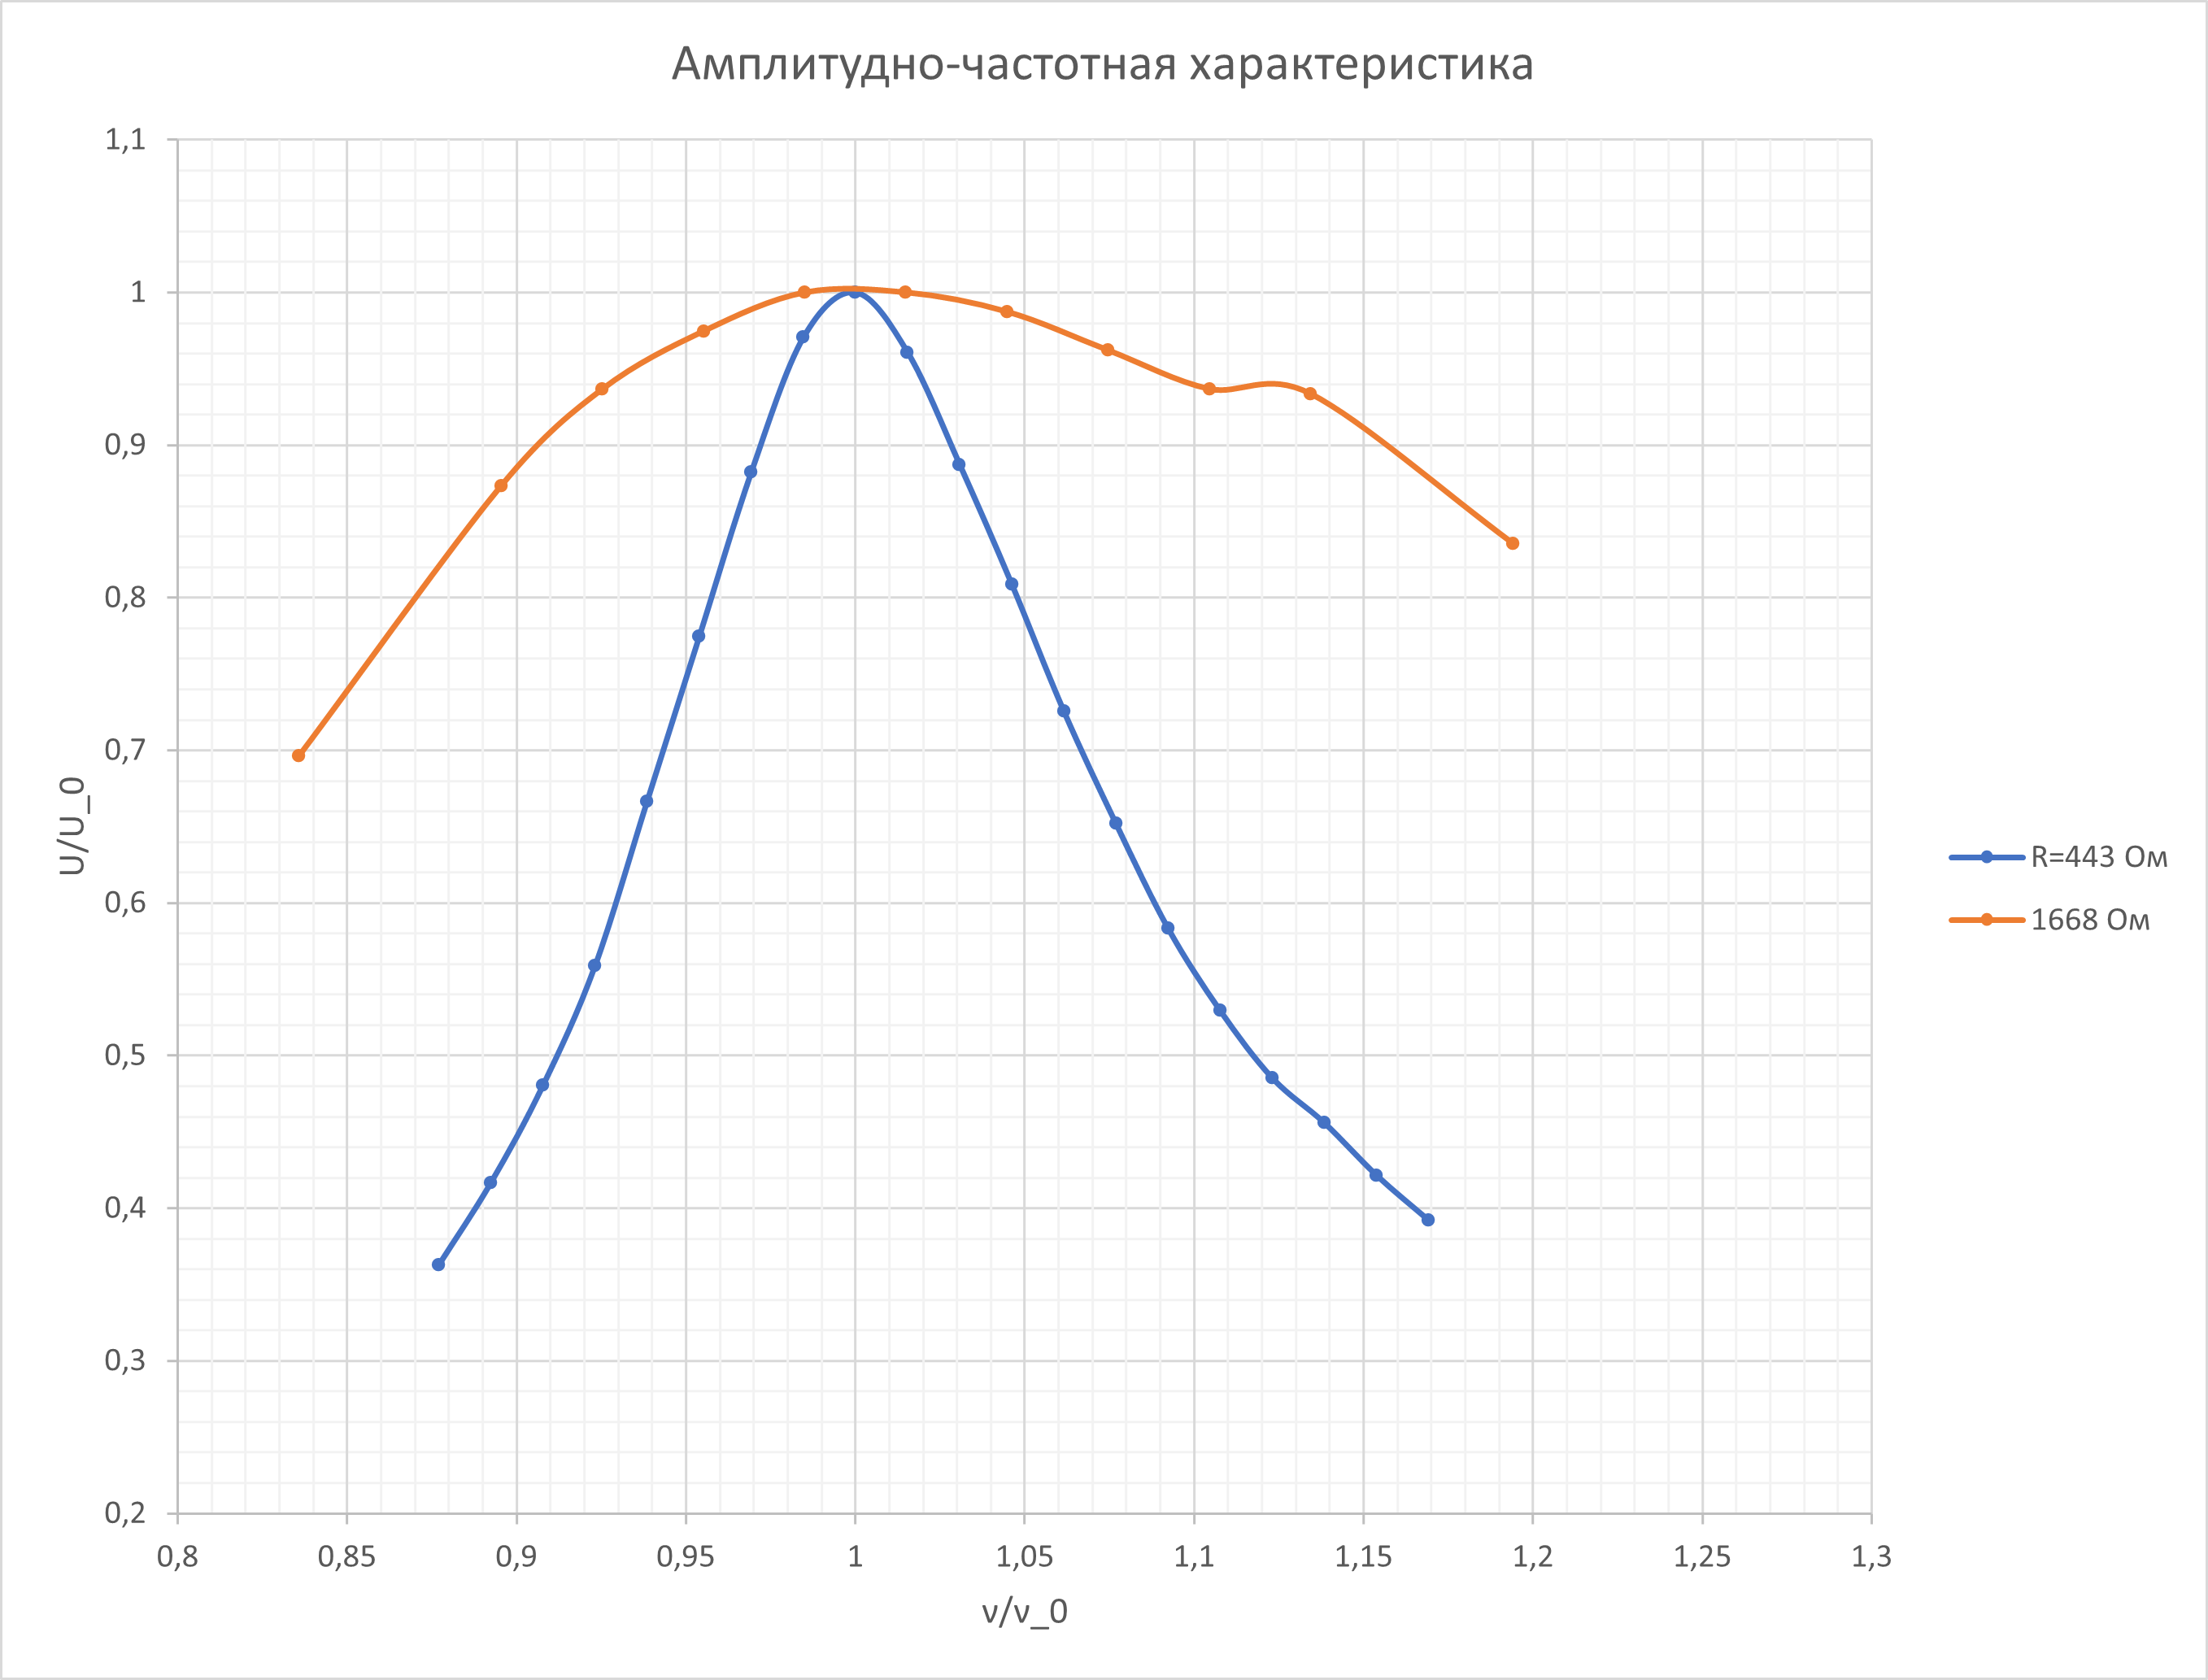
\includegraphics[width = \textwidth]{Gr3}
		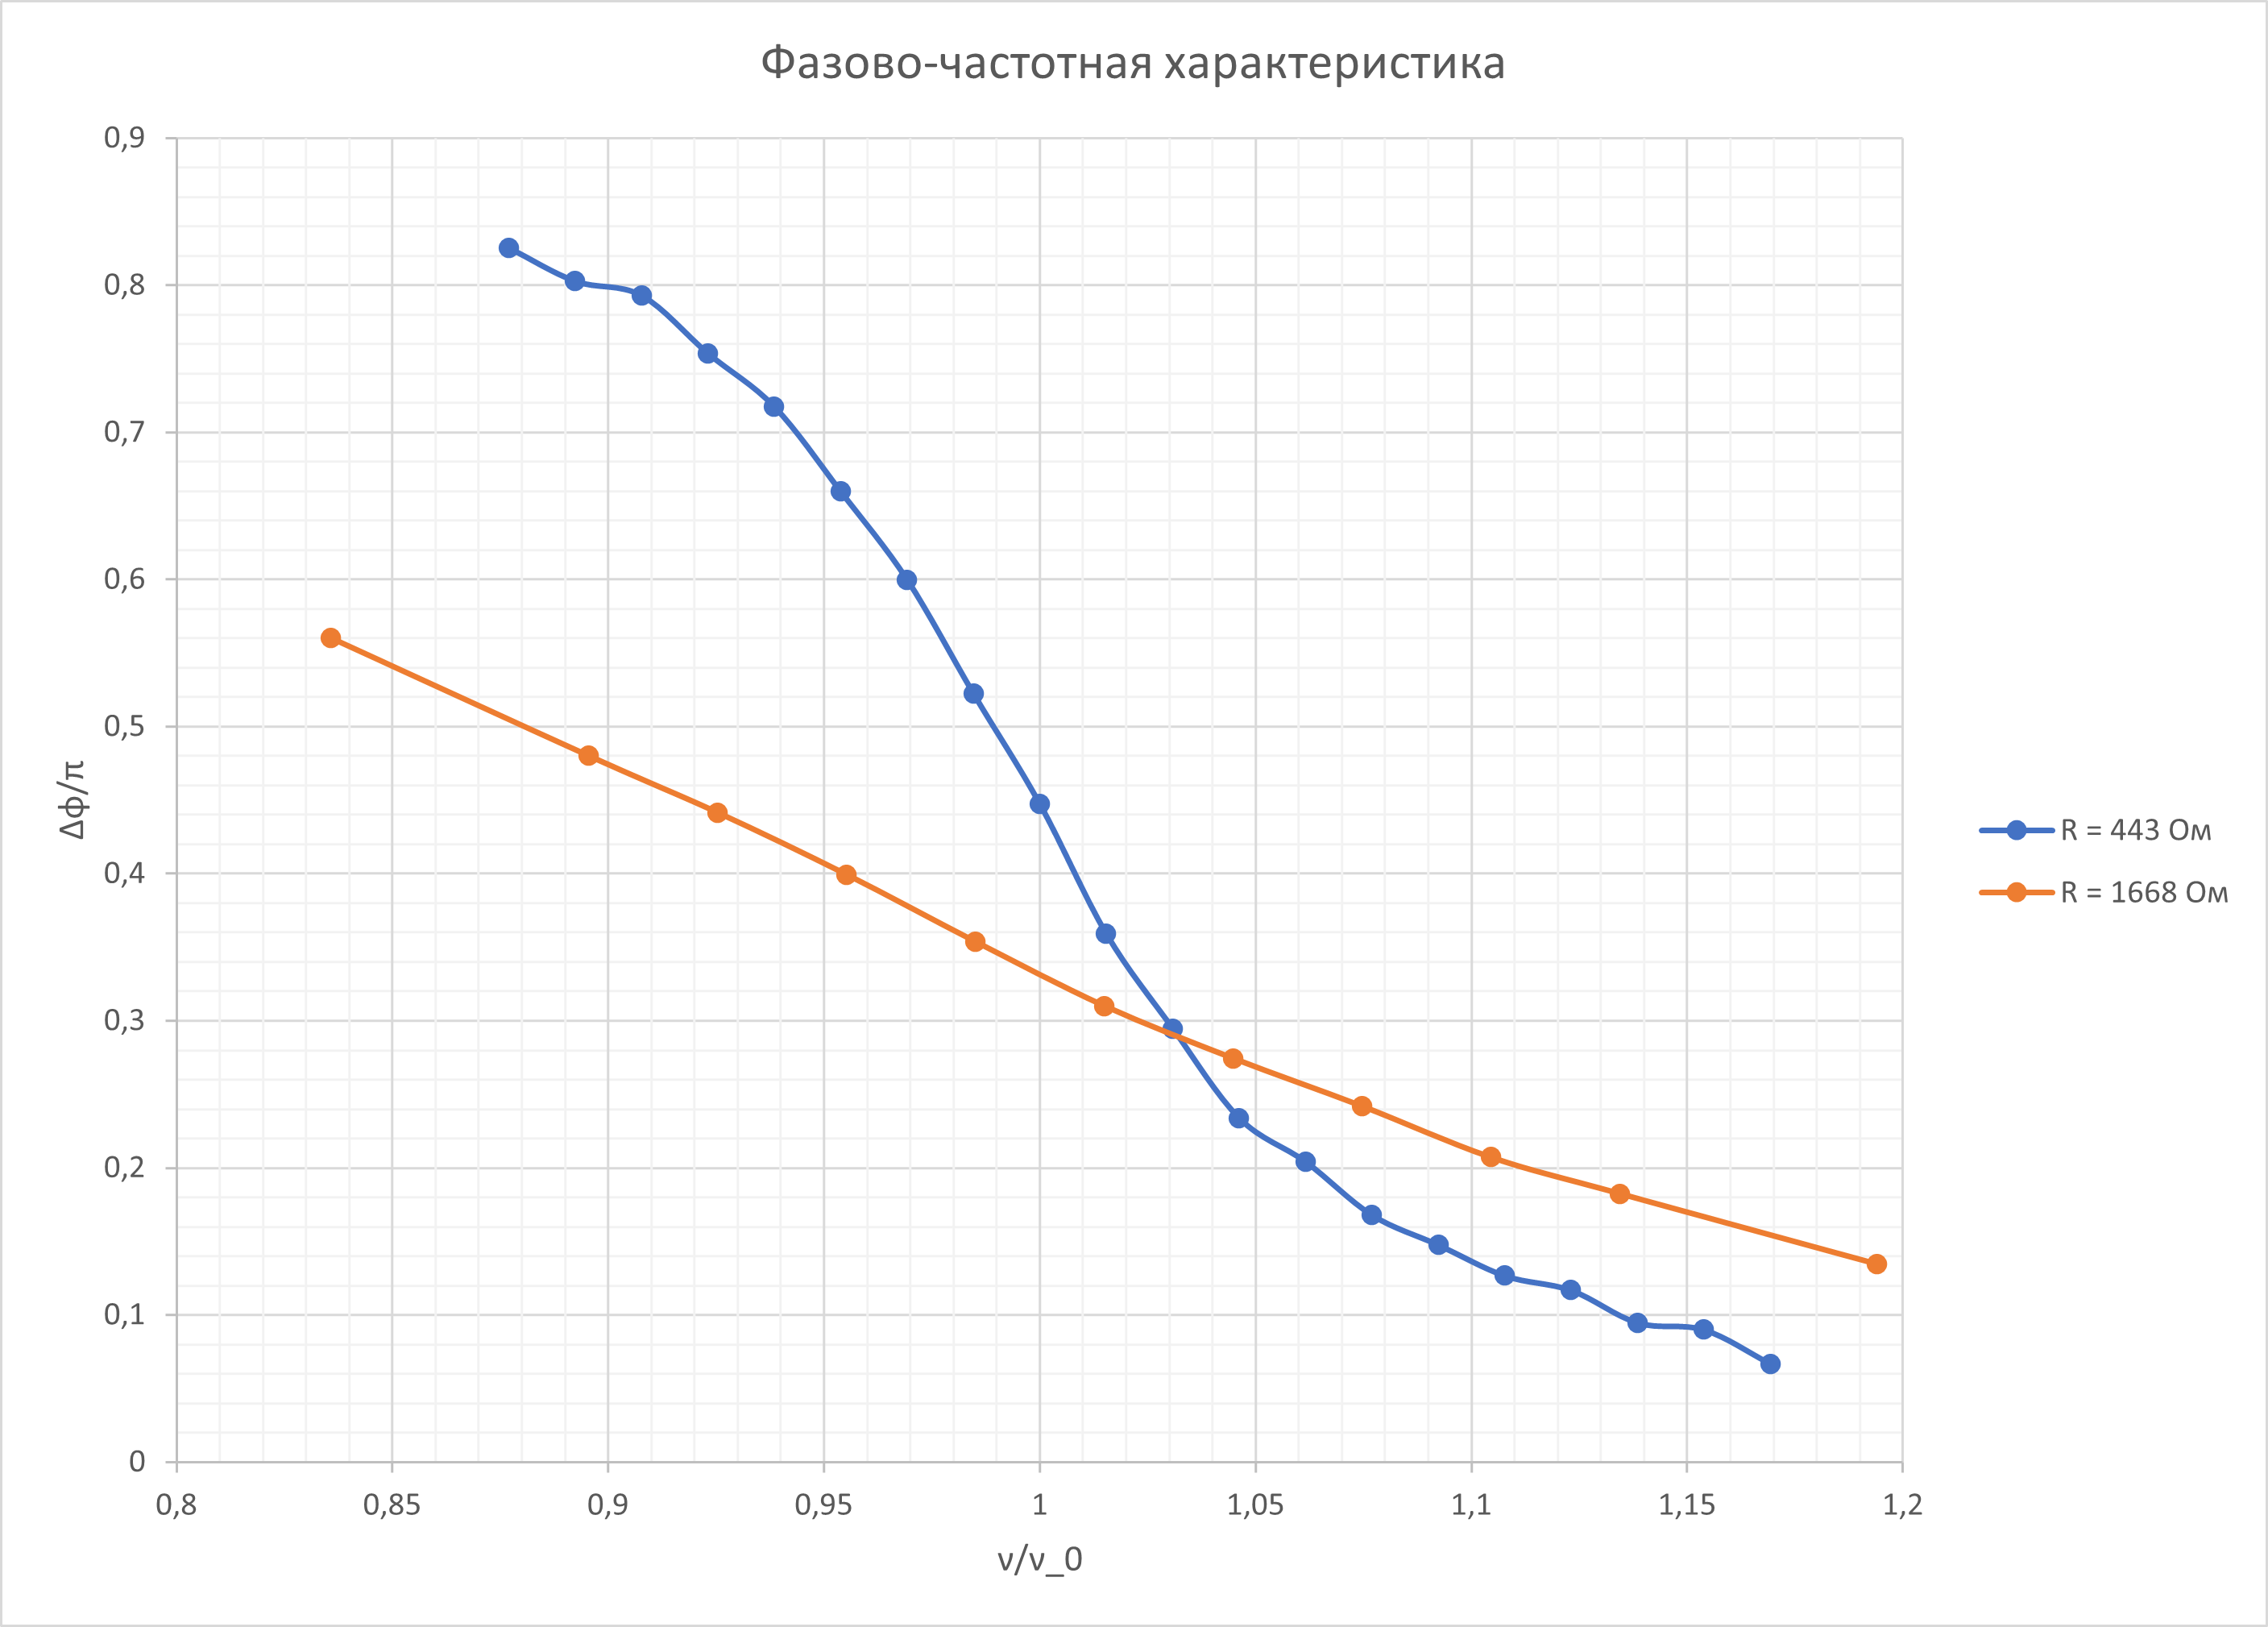
\includegraphics[width = \textwidth]{Gr4}
	\end{center}
	\newpage
	\begin{table}[h!]
		\centering
		\begin{tabular}{|c|c|c|c|}
			\hline
			$R$, Ом & $\frac{2\Delta \Omega}{\omega_0}$ & $Q$ & $\sigma_{Q}$ \\ \hline
			443 & 0,12 & 8,33 & 0,69\\ \hline
			1668 & 0,43 & 2,33 & 0,16 \\ \hline  
		\end{tabular}
		\caption{Определение добротности по графику АЧХ}
	\end{table}
	
	Определим добротность по графику АЧХ. $Q = \frac{\omega_0}{2\Delta \Omega}$, где $2\Delta \Omega$ - ширина резонансной кривой на уровне $U = \frac{U_0}{\sqrt{2}}$
	
	Рассчитаем добротность по ФЧХ. Для этого проведем горизонтальную линию через уровень, где наблюдается резонанс (ровно $\frac{\pi}{2}$ не наблюдается в экспериментальном резонансе). Затем отразим одну половину относительно этой прямой и измерим приблизительно ширину на расстоянии $\frac{\pi}{4}$ от резонанса (ровно в $\frac{\pi}{4}$ не сможем измерить ввиду недостатка точек и смещения резонанса).
	Примерные результаты:
	
	\begin{figure}[h]
		\centering
		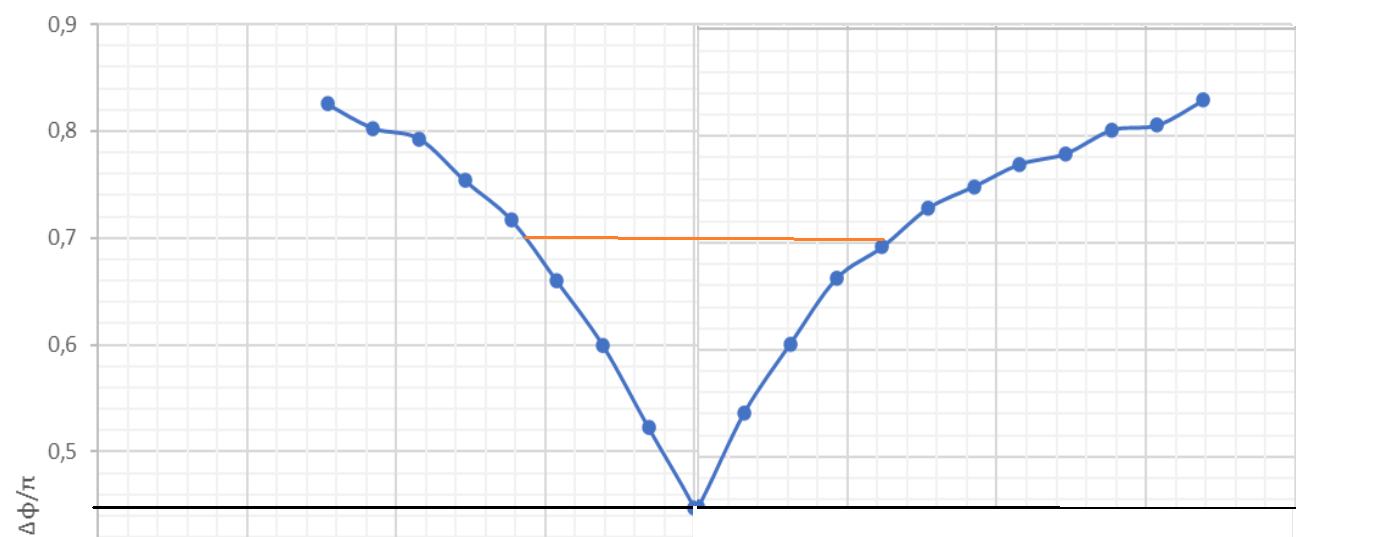
\includegraphics[width = \textwidth]{Gr6}
		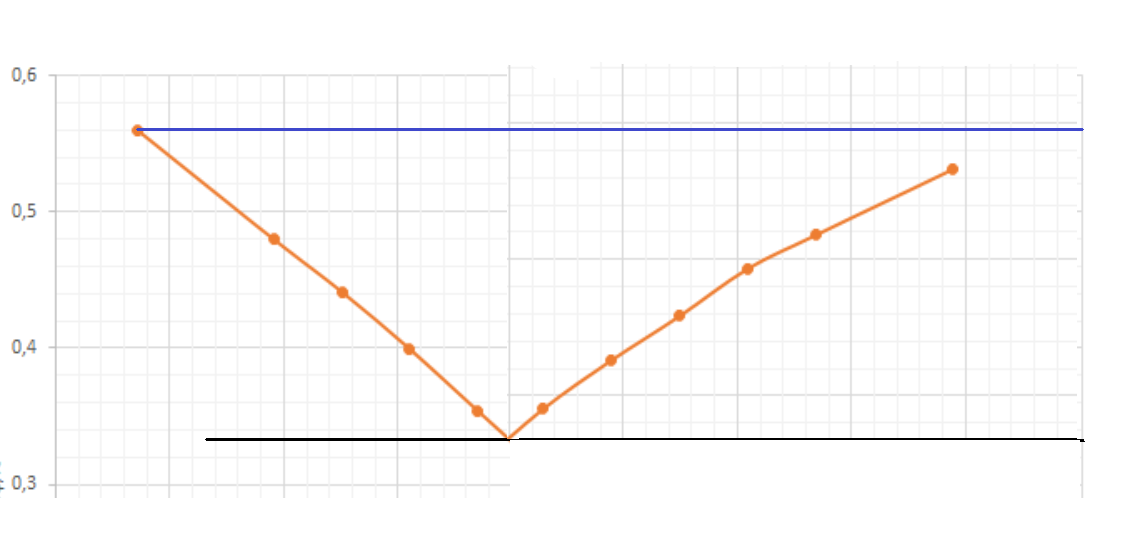
\includegraphics[width = \textwidth]{Gr5}
		\caption{Вспомогательные графики для определения погрешности по ФЧХ}
	\end{figure}
	
	\begin{table}[h]
	\centering
	\begin{tabular}{|c|c|c|c|}
		\hline
		$R$, Ом & $\frac{\Delta \omega}{\omega_0}$ & $Q$ & $\sigma_{Q}$ \\ \hline
		443 & 0,115 & 8,70 & 0,76 \\ \hline
		1668 & 0,415 & 2,41 & 0,17 \\ \hline  
	\end{tabular}
	\caption{Определение добротности по графику ФЧХ}
	\end{table}
	
	Погрешности в этих методах сложно оценить. Примем погрешность в определении ширины резонансной кривой за $\sigma_{\frac{\Delta \omega}{\omega_0}} = 0,01$ в случае $R = 443$ Ом и $0,03$ в случае $R = 1668$ Ом. (для второго случая приходится немного экстраполировать).
	
	\newpage
	\textbf{6.} Итоговая таблица:
	\begin{table}[h]
		\centering
		\begin{tabular}{|c|c|c|c|c|c|}
			\hline
			$R$, Ом & $f(L, C, R)$ & $f(\theta)$ & Фаз. спираль & АЧХ & ФЧХ \\ \hline
			443 & $9,20 \pm 0,10$ & $8,25 \pm 0,65$& $8,20 \pm 0,86$ & $8,33 \pm 0,69$ & $8,70\pm 0,76$ \\
			& $(1\%)$ & $(8\%)$ & $(10\%)$ & $(8\%)$ & $(9\%)$  \\ \hline
			1668 & $2,40 \pm 0,01$ & $ 2,46 \pm 0,06$ & $ 2,35 \pm 0,18$ & $2,33 \pm 0,16  $ & $2,41 \pm 0,17 $ \\
			& $(0,3 \%)$ & $(2\%) $ & $(8\%) $ & $(7 \%) $ & $(7 \%) $ \\ \hline
		\end{tabular}
	\end{table}
	
	\subsection*{Вывод}
	 В данной лабораторной работе мы исследовали свободные и вынужденные колебания в электрическом контуре и различными способами находили его добротность. Самый точный способ, конечно же, теоретический. Затем достаточно эффективен способ вычисления через декремент затухания. Фазовая спираль даёт высокую погрешность, поэтому это не очень надежный способ вычисления добротности. Способы вычисления через АЧХ и ФЧХ хороши, если есть специальная программа, позволяющая вычислять ширину резонансной кривой, и хорошо снятые данные (с этим тоже возникли проблемы). Несмотря на то, что при нашей оценке у $R_2 = 1668$ Ом относительная погрешность в этих опытах $7 \%$, данные были сняты некачественно и ориентироваться на них сложно.
\end{document}